\section{Conceptos b�sicos de hidr�ulica urbana en RDA}
Conjunto de elementos enlazados de tal manera que permite suministrar cierta cantidad de agua a una presi�n establecida~\cite{Doctoral2012}.

\paragraph{Presion:} Fuerza ejercida sobre una superficie.
\paragraph{Caudal:} Cantidad de agua que se mueve a trav�s de un segmento de la red.
\paragraph{Factor de fricci�n:} Coeficiente adimensional que especifica la rugosidad de la tuber�a~\cite{Perez-2011}.
\paragraph{Curva de consumo:} Gr�fica del consumo en un periodo de tiempo.

\subsection{Componentes f�sicos de una red}
A continuaci�n se define los componentes que conforman una red de agua potable~\cite{Rossman2017}, los cuales se aprecian en la Figura~\ref{fig:componentesfisicos}:


\begin{figure}[h]
	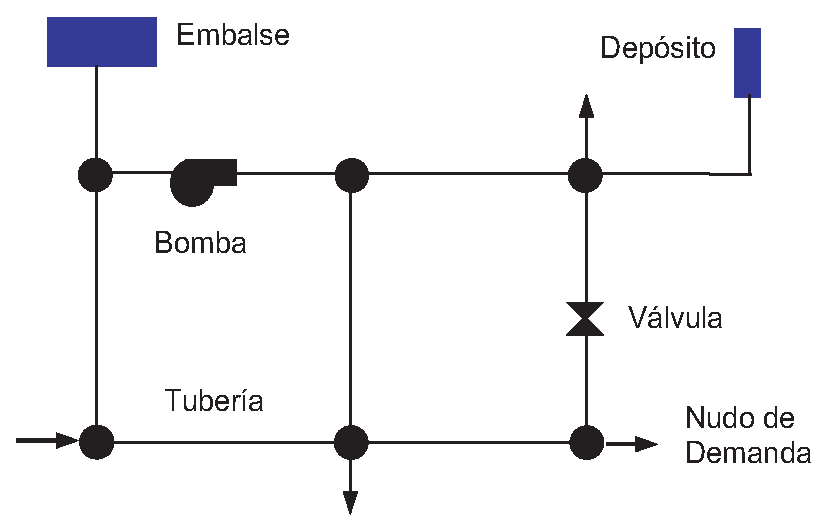
\includegraphics{Capitulo2/assets/componentesfisicosred.eps}
	\centering
	\caption[Componentes f�sicos de un sistema de distribuci�n de agua]{Componentes f�sicos de un sistema de distribuci�n de agua~\cite{Rossman2017}}
	\label{fig:componentesfisicos}
\end{figure}
\paragraph{Nudos de consumo:} Son los puntos o extremos de una tuber�a, los cuales tambi�n permiten que estas se unan. Estos nudos pueden actuar como nudos de demanda a trav�s de los cuales el flujo abandona la red.

\paragraph{Reservorio:}Es una fuente de alimentaci�n externa.
\paragraph{Deposito:}Son elementos con la capacidad de almacenar agua.
\paragraph{Tuberias:}Son los elementos a trav�s de los cuales transita el agua de un nudo a otro.
\paragraph{Bombas:}Elementos que permiten impulsar el liquido con el fin de elevarlo a una posici�n superior.
\paragraph{V�lvulas:}Elementos que limitan la presi�n o el caudal que transita en un punto de la red.